\subsection{Algemeen concept}
De testen maken gebruik van een simpele server waar clients op kunnen verbinden. De client kan vervolgens het absolute tijdverschil meten met een atomische wereldklok.

Eerst en vooral is er een vertraging tussen een aangesloten client en de server, de {\it ping}. Dit is gemeten in milliseconden. De testen meten de vertraging door een bericht met de actuele tijd te verzenden van de server naar de client, en terug. De vertraging is dan de verzonden tijd afgetrokken van de actuele tijd waarmee de ping verkregen is.
In figuur \ref{ping} is de informatieoverdracht zichtbaar. De server berekent de servertijd (TS1) door middel van een API die de exacte wereldtijd teruggeeft, verzonden naar de client en teruggekregen. De uiteindelijke ping is: \[ping = TS2 - TS1\] met TS2 de actuele tijd berekent in de server TS2

\begin{figure}[h]
\centering
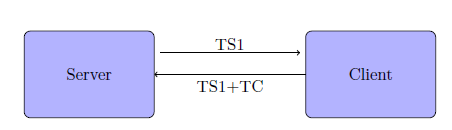
\includegraphics[scale=0.8]{img/img.png}
\caption{Ping} \label{ping}
\end{figure}


Het is niet gegarandeerd dat de klokken van de clients allemaal gesynchroniseerd zijn met de server. Bij het terug verzenden van de client naar de server wordt de clienttijd (TC) bij het bericht gezet.  Met deze TC en de berekende {\it ping} is het mogelijk het tijdsverschil tussen de client en de server te bepalen ($DeltaTime$).
\[DeltaTime = (TC+ping/2) - TS2\]
Het verslag zal deze data bekijken vergelijken tussen verschillende browsers en besturingssystemen.

\subsection{UDP vs TCP}

UDP heeft in tegenstelling tot TCP geen verbinding nodig tussen bijvoorbeeld server en client. TCP zal garanderen dat data correct aankomt door middel van foutopsporing en zal ook in de goede volgorde binnenstromen. Om geen pakketten te verliezen zal TCP deze in een {\it receive buffer} steken en zal de applicatie de ontvangen data pas lezen als ze er klaar voor is. Tegenover UDP waar de data continu zal binnenstromen, ontvangen of niet. Deze zal ook niet aan foutopsporing doen en de juiste volgorde is niet gegarandeerd. Het is duidelijk dat UDP veel sneller is doordat deze minder stappen bevat. Het UDP is dan effectief sneller dan het TCP protocol. Nochtans is het niet mogelijk het UDP protocol te gebruiken omdat browsers deze functionaliteit niet bevatten. Daarom is er nu gebruik gemaakt van Socket.io dat met het TCP protocol werkt.

\subsection{Drift en skew}

Drift zal ervoor zorgen dat een klok uit sync valt met een referentie. Windows lost dit op met een wekelijkse resync (het tijdsverschil zal dus op een sawtooth diagram lijken) terwijl Mac OSX rekening zal houden met de klok skew om zo beter in sync te blijven.
Klok skew is het verschil van tijd van een klok signaal tussen 2 componenten (zie figuur \ref{skew1} \cite{skew}).

Het tijd verschil van een windows computer en een atoom clock is gedurende 25 minuten gemeten (zie figuur \ref{drift}). De trendlijn is door de grafiek getrokken en het is duidelijk dat er al dan niet geen effect ervan te zien is. Over langere tijd periode zal de drift groter worden maar voor de animatie zal dit verwaarloosbaar zijn aangezien het onwaarschijnlijk is dat iemand dagenlang zal blijven spelen.

\begin{figure}[H]
\centering
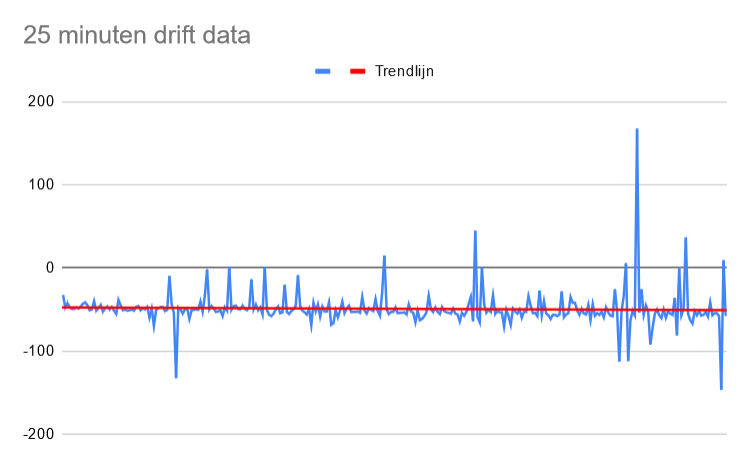
\includegraphics[scale=0.3]{img/drift.png}
\caption{Drift} \label{drift}
\end{figure}

\begin{figure}[H]
\centering
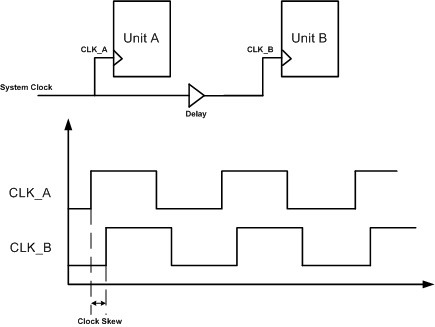
\includegraphics[scale=0.7]{img/skew.jpg}
\caption{Skew} \label{skew1}
\end{figure}


Klok skew kan problemen geven voor correct timings, en zoals eerder vermeld zal OSX dit tegen gaan via software. We zullen niet dieper gaan over de problemen van skew en OSX. 


\subsection{Analyse van de data}
Als premise is er gesteld dat de aangesloten clients gesynchroniseerd zouden zijn met de wereldklok, gebruikmakend van het interne synchronisatie systeem op elk toestel. Het is duidelijk in figuur \ref{fig:mediaan} dat er op elk soort systeem een afwijking gemeten wordt tegenover de referentieklok. Bij sommige operating systems al een groter verschil dan de andere, maar de reden waarom is niet altijd te verklaren of vrijgegeven en zullen hier dus niet verder op in gaan. Om dit te testen is er een poging gedaan om het verschil tussen device-klok en server-klok te vergelijken door de ping mee in rekening te brengen. De drift van beide klokken gaan over deze tijdsspanne minimaal zijn en gaan geen invloed hebben op deze verschillen. Bij de testen werd ook de gemiddelde ping en standaarduitwijking van de ping per test opgeslagen. Uit deze waarden valt af te leiden dat er bij grote ping fluctuaties ook een grote standaarduitwijking mee gepaard ging en wijst naar inconsistenties binnen het netwerk van ofwel de client ofwel de belasting op de server en is er bijgevolg meer kans op een grotere fout binnen de vergelijking van de klokken.

\begin{figure}[H]
	\centering
	\begin{subfigure}{.5\textwidth}
		\centering
		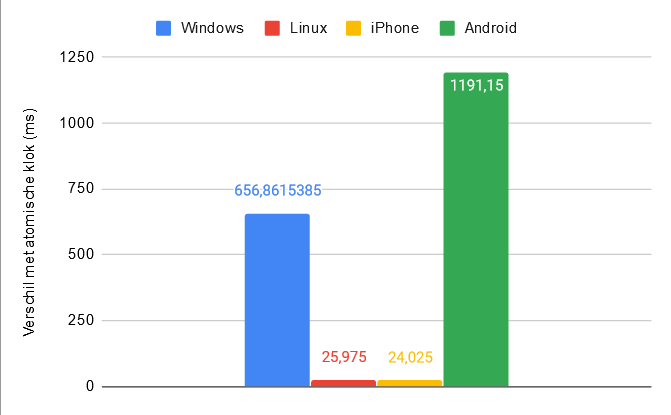
\includegraphics[width=.95\linewidth]{img/mediaan.png}
		\caption{Mediaan van tijdsverschil van elk device.}
		\label{fig:mediaan}
	\end{subfigure}%
	\begin{subfigure}{.5\textwidth}
		\centering
		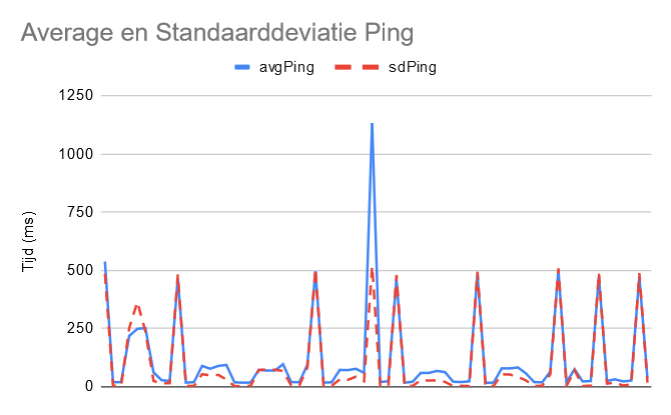
\includegraphics[width=.95\linewidth]{img/ping_results.png}
		\caption{Gemiddelde en standaarduitwijking van de ping met de server. }
		\label{fig:avgPing}
	\end{subfigure}
	\caption{Resultaten van de testen}
	\label{fig:results}
\end{figure}

In figuur \ref{fig:avgPing} is het duidelijk zichtbaar dat er een pieken zijn met hoge standaardafwijkingen. Dit wilt zeggen dat er heel grote fluctuaties zijn in de ping tijdens het synchronisatie proces met 10 metingen. Hiermee zal de gesynchroniseerde tijd een afwijking hebben met de werkelijke tijd tot +-($maxPing - minPing$) milliseconden.




















